\section{Увод}

Приликом развоја оперативних система, драјвера, \verb|bootloader|-а и других критичних системских софтвера, користе се језици ниског нивоа као што су \verb|C| и \verb|C++|.
Током година \verb|Microsoft| је увидео да је преко 70\% безбедносних слабости настало неадекватним руковањем меморијом \cite{msrc}. Најчешћи примери су коришћење меморије 
након ослобађања, вишеструко ослобађање исте меморијске локације, небезбедна аритеметика показивачима, цурење меморије и препопуњавање бафера.
Такође са становишта паралелног програмирања, оба језика захтевају педантно руковање мутексима и семафорима јер у супротном настају нови проблеми попут 
проблема трке и проблема међусобног чекања. Проблем трке настаје када две или више нити покушавају да измене податак истовремено, при чему редослед извршавања 
утиче на исход. Проблем међусобног чекања настаје када две или више нити чекају једну на другу да ослободе ресурсе при чему се извршавање 
зауставља.

Програмски језик \verb|C| нема уграђене одбрамбене механизме од претходно наведених проблема. Придржавање \verb|C| стандарду отвара могућност за упоредо 
коришћење \verb|GCC| и \verb|Clang| компајлера чиме се добија увид у релативно штура упозорења од стране оба програмска преводиоца.
Са друге стране програмски језик \verb|C++| упркос додавању примитива као што су \verb|unique_ptr|, \\ \verb|shared_ptr| и \verb|weak_ptr|, и даље због интероперабилности 
са старијим стандардима или библиотекама захтева коришћење сирових показивача. Временом су се развили софтверски обрасци као што је \verb|scope|-\verb|bound| \verb|resource| \verb|management|
које настоји да добрим праксама умањи шансу да се проблем првобитно деси. Наиме, корисник језика није приморан да софтверски образац употреби или чак зна 
за његово постојање.

\verb|Rust| је програмски језик створен са јасним циљем: да реши проблеме повезане са меморијском и паралелном безбедношћу. 
Његова подразумевана употреба гарантује безбедност захваљујући робустом систему типова, иновативном начину управљања меморијом и стриктног \verb|rustc| компајлера.
За разлику од \verb|C| и \verb|C++| који често дају нејасне поруке о грешкама, \verb|Rust| нуди изузетно прецизне дијагностичке поруке које тачно указују на место 
грешке и нуде потенцијална решења.

Са обзиром на значајне иновације које доноси \verb|Rust| језик, детаљно разумевање његовог интерног функционисања је од великог значаја. \verb|Rust|-ове гаранције 
безбедности нису магичне, примарно произилазе из система правила \verb|borrow-checker|-а, животних векова и особина које гарантују безбедност неког типа 
у паралелном окружењу. \verb|Rust| нуди многе напредне функције као што су макрои, небезбедан код, \verb|FFI| за интеракцију са \verb|C| кодом. Детаљно разумевање основа језика и његовог интерног функционисања је предуслов за ефикасно коришћење ових напредних 
могућности на сигуран и ефикасан начин. На пример, када се користи \verb|unsafe| блок, програмер преузима одговорност за безбедност меморије, 
што захтева дубоко разумевање начина на који \verb|Rust| обично то ради.

Занимљиво је да је прва верзија \verb|Rust| компајлера била написана у \verb|O'Caml|-у, али су све наредне верзије развијене у самом \verb|Rust|-у. 
Важно је напоменути да је \verb|Rust| заправо само фронтенд за \verb|LLVM|. \verb|LLVM| представља скуп модуларних и вишекратно употребљивих технологија за изградњу компајлера. 
\verb|Rust| се у потпуности ослања на \verb|LLVM| за генерисање машинског кода, док је комплетан фронтенд \verb|Rust|-а написан од нуле.

Међурепрезентације изворног кода у \verb|Rust|-у обухватају различите приказе корисничког кода који омогућавају кључне функционалности језика, 
укључујући проверу типова, дијагностику грешака, аутоматску деалокацију меморије и друге ергономске и функционалне карактеристике.

\newpage

\section{Позадина}

У овој секцији обрађује се позадина иза \verb|Rust| језика, званичног менаџера пакета \verb|Cargo| и 
\verb|LLVM| сета алата.

\subsection{Rust језик}

\verb|Rust| је статички типизиран језик који је настао 2006. године као лични пројекат \verb|Graydon| \verb|Hoare|-а, радника компаније 
\verb|Mozilla|. Увидевши потенцијал језика, \verb|Mozilla| је започела спонзорисање пројекта 2010. године када је језик и јавно 
представљен \cite{rust-language}. \verb|Rust| је језик ниског нивоа који се фокусира на меморијску безбедност
и безбедан паралелизам без ослањања на скупљач смећа (\verb|garbage| \verb|collector|). Скупљач смећа 
обично уводи лакоћу програмирања на уштрб недетерминистичких перформанси услед ослобађања меморије 
са \verb|heap|-а, на меморијским локацијама где је бројач референци на нули. У језицима без скупљача 
смећа обично постоји одредба која се позива да би се динамички алоцирана меморија ослободила. \verb|Rust|
језик уводи сасвим нови концепт у домен програмских језика, позајмљивач (\verb|borrow| \verb|checker|).
Позајмљивач се заснива на стриктној примени менаџмента ресурса у опсегу (\verb|scope-bound| \verb|resource| \verb|management|) 
од стране компајлера. Ово је софтверски образац који је препоручљиво користити у небезбедним језицима 
ниског нивоа. Наиме у природи софтверског обрасца јесте да га није могуће приморати, осим ако није директно
интегрисан у језик као што је случај са језиком \verb|Rust|. Кључан концепт који се уводи уз позајмљивач 
јесте власништво. Власништво представља дужност да опсег који директно манипулише меморијом (приступ меморији није 
придобијен референцом) ту меморију на крају опсега ослободи. 

У језику \verb|C| постоје два начина дељења 
меморије: преко вредности и преко референце (показивача). Дељење преко вредности (копија) је
подразумевано. У \verb|Rust|-у дељење преко вредности није подразумевано понашање, већ је основна акција пренос власништва.
Дељење преко вредности се може симулирати клонирањем (функција \verb|clone|) коју прати пренос власништва.
Опсег у коме је меморија додељена варијабли валидна 
се назива животни век. Власништво онемогућује бројне грешке као што су коришћење након ослобађања и цурење 
меморије тј. активно врши забрану недефинисаних стања. Програм се не компајлира успешно уколико правила 
власништва нису задовољена. Изворни код \ref{lst:use_after_free_c} представља \verb|C| код који користи меморију 
након ослобађања. Успешно се компајлира али приликом извршавања враћа грешку. Са друге стране у изворном 
коду \ref{lst:user_after_free_rust} представљен је исти концепт у \verb|Rust| језику. Функција 
\verb|drop| преузмима власништво над меморијом 
и ослобађа је, симулирајући крај опсега. Изворни код \ref{lst:user_after_free_rust} се неће 
успешно компајлирати јер се врши покушај манипулацијом меморије над варијаблом којој је прошао животни век.
Уједно је демонстрирано да корисник \verb|Rust| језика не мора да се стара о животном веку варијабле, искључујући
цурење меморије као опције.

\begin{multicols}{2}
    \begin{listing}[H]
    \begin{minted}{C}
int* pointer = malloc(sizeof(int));
*pointer = 5;
pointer = NULL;
free(pointer);
*pointer = 6; 
    \end{minted}
    \caption{Коришћење након ослобађања - C}
    \label{lst:use_after_free_c}
    \end{listing}
    \columnbreak
    \begin{listing}[H]
    \begin{minted}{rust}
let mut a: Box<i32> = Box::new(5);
drop(a);
*a = 6;
    \end{minted}
    \caption{Коришћење након ослобађања - Rust}
    \label{lst:user_after_free_rust}
    \end{listing}
\end{multicols}

У језику \verb|C++|, добра пракса је правилно означавати непроменљивост референце или вредности
унутар функција коришћењем кључне речи \verb|const|, обавештавајући будућег корисника функције 
о променљивости. У језику \verb|Rust|, променљивост мора да се назначи експлицитно употребом кључне 
речи \verb|mut|. Инверзија принципа је омогућила далеко бољу читљивост и разумевање кода.

Безбедни паралелизам је једна од главних одлика \verb|Rust| језика. Реализује се помоћу особина (\verb|trait|)
и власништва. Особине су уговор који се поставља над структуром и по функционалности личе на интерфејсе
у другим језицима. Главна разлика је у флексибилности. Особине могу да се имплементирају над типовима
које нисмо ми дефинисали, на пример из других библиотека. Разлог томе јесте баш у кључној речи уговор.
Ако структура задовољава уговор који особина налаже (обично испуњење других особина или
метода) онда је особина применљива над структуром. Кључне особине које реализују безбедност података
у паралелном окружењу јесу \verb|Sync| и \verb|Send|. Тип је \verb|Send| ако је безбедно послати га 
у другу нит. Тип је \verb|Sync| ако га је безбедно делити између нити. Типови сачињени од других типова који
имплементирају \verb|Sync| и/или \verb|Send| су аутоматски \verb|Sync| и/или \verb|Send|. Скоро све примитиве
унутар \verb|Rust| језика су \verb|Send| и \verb|Sync|. У битније изузетке спадају сирови показивачи јер немају
безбедносне гаранције, \verb|UnsafeCell| (самим тиме и \verb|Cell| и \verb|RefCell|) јер имплементирају
унутрашњу мутабилност чиме је тип ризик у виду штетног преплитања, као и \verb|Rc| (бројач референци) 
јер је број референци дељен и несинхронизован. Уз \verb|std::marker|, \verb|Sync| и \verb|Send| су једине особине које су 
део самог компајлера, а не стандардне библиотеке.

Атрибути су заглавља која пружају додатне информације компајлеру. Атрибути могу бити спољашњи или 
унутрашњи \ref{lst:attributes}. Примењују се на бројне конструкте унутар језика као што су екстерни блокови,
функције, модули и енумерације. Атрибути генеришу код, искључују или укључују дијагностику, 
постављају лимитације и уделују у тестирању. 

\begin{listing}[H]
\begin{minted}{rust}
// Spoljašnji atribut se primenjuje na tip koji sledi 
// nakon atributa koji pri tome nije atribut.
#[allow(dead_code)] 
fn main() {
    // Unutrašnji atribut.
    // Primenjuje se na vlasnika lokalnog opsega. 
    #![allow(unused_variables)]
    let x = 10;  
}
\end{minted}
\caption{Спољашњи и унутрашњи атрибути}
\label{lst:attributes}
\end{listing}

Макро систем је један од најмоћнијих делова \verb|Rust| језика. Макрои су код који генерише други код и овај 
начин програмирања се назива метапрограмирање. 
Корисни су да би се смањила количина кода која мора да се одржава, али и да би се избегло вишеструко писање 
веома сличног кода (\verb|boilerplate|). Постоји четири врсте макроа: декларативни, функцијски, процедурални и атрибутски. 
Декларативни и функцијски су слични по природи, позивају се налик обичним функцијама али у именовању имају суфикс "!".
Декларативни макрои морају детерминистички навести број параметара, док функцијски имају произвољан број параметара.
Један од најчешће коришћених декларативних макроа јесте \verb|vec!| који служи да смањи број линија кода да би се 
иницијализовао вектор. Са друге стране функцијски макрои могу да се користе да би се писала синтакса неког другог језика, 
што је и честа појава у \verb|Rust| библиотекама које позивају \verb|SQL| или \verb|Python|.
Процедурални макрои су макрои који увозе кроз предефинисани \verb|derive| атрибут, док атрибутски макрои генеришу сасвим 
нови атрибут. Главна разлика између њих јесте у флексибилности. Процедурални макрои раде на структурама и енумерацијама,
док атрибутски макрои могу бити дефинисани да раде и над другим ставкама језика попут функција.

\verb|Rust| језик се одликује апстракцијама без цене. Особина апстракција без цене означава да концепти 
вишег нивоа као што су колекције и генерички типови не утичу на перформансе програма приликом његовог извршавања.
\verb|Rust| омогућава ову карактеристику путем мономорфизације. Мономорфизација је процес путем којег се креира 
копија генеричког кода за сваки конкретан тип који користи генерички код тј. генерички код се претвара у 
негенерички код. Наиме овај процес повећава величину крајњег извршног фајла и продужава време компајлирања.
Генеричке структуре могу да имају највећи утицај на величину извршног фајла. Проблем се амортизује 
тако што се не генеришу методе за конкретан тип ако их исти не користи у изворном коду.


\newpage
\subsection{Cargo}

У \verb|Rust|-у, \verb|Crate| је најмања јединица организације кода. Постоје два основна типа, извршни програми и библиотеке.
Извршни програми садрже \verb|main| функцију и могу да се извршавају. Библиотеке се не извршавају и немају потребу за \verb|main|
функцијом већ пружају функционалности које се могу користити у другим \verb|Crate|-овима. 

Скоро сваки модрени језик долази са једним или више менаџера пакета (библиотека). Званични менаџер пакета у \verb|Rust|
екосистему се назива \verb|Cargo|. Главни задатак му је да бележи зависности програма тако да је могуће рекреирати 
програм на детерминистички начин. Уводе се \verb|Cargo.lock| и \verb|Cargo.toml|
фајлови. \verb|Cargo.toml| је манифест фајл који одржава корисник. Састоји се мета података попут назива и верзија као и списка пакета са кориснички дефинисаним 
верзијама (или опсегом верзија) који се тренутно користе у програму. Поред верзије, пакети могу да имају функционалности које корисник мора експлицитно да наведе уколико су потребни.
\verb|Cargo.lock| се генерише након корака компајлирања али га је могуће изгенерисати кроз \verb|cargo| \verb|generate-lock| команду.
\verb|Cargo.lock| омогућава да се при компајлирању програма на потеницјално различитим машинама користе идентични пакети праћењем тачне верзије сваког појединачног пакета.

\verb|Cargo| добавља зависности из регистра. Регистар садржи индекс у коме се налази листа доступних \verb|Crate|-ова. Подразумевани јавни регистар је \verb|crates.io|, али је могуће 
конфигурисати сопствени регистар који је произвољне видљивости. Један \verb|Crate| може користити зависности из различитих регистара. Уколико се \verb|Crate| налази у регистру који није 
подразумевани у \verb|Cargo.toml| фајлу се за ту зависност дефинише \verb|registry| атрибут.

\verb|Cargo| је отпорнији од менаџера пакета из других екосистема јер није могуће брисати верзије једном када је пакет објављен на јавном регистру. 
Овај приступ спречава нападе ланца снабдевања као што се десило у \verb|JavaScript| менаџеру пакета \verb|NPM|. Пакет \verb|left-pad| 
је сачињен од 11 линија кода који додаје специфицирану количину размака са леве стране низа карактера. Иако је пакет тривијалан, многе библиотеке које 
су масивно коришћене су директно или индиректно зависиле од њега. Проблем је настао када је креатор \verb|left-pad| пакета обрисао 
пакет са репозиторијума пореметивши огроман део екосистема. У софтверу отвореног кода напади ланца снабдевања постају све чешћи (преко 700\% повишена учесталост
из године у годину) и због тога регулаторне управе раде на стандардизацији менаџера пакета не би ли се овакви напади спречили \cite{supply-chain}.

Некада је \verb|Crate|-у неопходно да компајлира или \verb|link|-ује неки код који није написан у \verb|Rust|-у, на пример \verb|C| код. Користећи посебан фајл \verb|build.rs| у коренском директоријуму 
пројекта могуће је дефинисати скрипту коју ће \verb|rustc| да компајлира и изврши пре компајлирања циљаног \verb|Crate|-а. Подразумевано је да се скрипта извршава пред сваку компилацију,
али је могуће дефинисати путању или променљиву окружења приликом чије промене ће се скрипта поново (следећи пут када се компајлира \verb|Crate|) извршавати.

\verb|Cargo| поред дистрибуирања пакета пружа разне олакшице и аутоматизације у односу на сирово коришћење \verb|Rust| компајлера. 
Команда \verb|cargo init| се користи да би се једноставно иницијализовао нови \verb|Crate| заједно са \verb|Cargo.toml| фајлом. 
Команде \verb|cargo| \verb|add| и \verb|cargo| \verb|remove| додају и бришу пакет из \verb|Cargo.toml| фајла.
Команда \verb|cargo| \verb|check| компајлира тренутни \verb|Crate| без генерације кода (без употребе ЛЛВМ-а) што је значајно брже 
од покретања \verb|cargo| \verb|build| који и генерише код. Ово је корисно јер је већински део дијагностике заснован 
на корацима пре генерисања кода. Команда \verb|cargo| \verb|run| констрише пакет и извршава га. Ово је значајно јер у већини случајева корисник жели да покрене програм након што је 
написао измену и избегава \verb|CLI| гимнастику доласка до \verb|/target| фолдера и покретања извршног фајла. 
Команда \verb|cargo| \verb|test| покреће све \verb|unit| тестове који се дефинишу употребом атрибута \verb|test| над функцијама.
Будући да је \verb|Cargo| делом апстракција над \verb|rustc| компајлером и да је \verb|rustc| изузетно конфигурабилан, користи се команда \verb|cargo| \verb|rustc|
која прима додатне компајлерске опције.

\newpage

\subsection{LLVM пројекат}

Генерисање кода је један од најтежих задатака приликом креирања новог компајлера. Изворни код који 
корисници пишу се преводи у машински код и пре свега мора бити тачан. Поред тачности циљ приликом 
дизајнирања генератора кода јесте лака имплементација, тестирање и одржавање.
Приликом превођења обично постоји 
више међу репрезентација изворног кода са циљем да валидира и оптимизује изворни код. Међу репрезентације 
се сврставају у \verb|frontend| или у \verb|backend|. \verb|Frontend| има за задатак да скенира, парсира 
и преведе изворни код у релативно ниску међу репрезентацију. \verb|Backend| стога може да претпостави 
да су све статичке синтактичке и семантичке грешке детектоване и да су типови и њихове конверзије
обрађене на основу чега оптимизује и генерише код за циљану архитектуру.

\verb|LLVM| пројекат је скуп модуларних и поново искористивих компајлерских технологија \cite{llvm}. Под окриљем \verb|LLVM|-а
се налазе бројни пројекти. Главни пројекат је \verb|LLVM| \verb|Core| унутар кога је специфицирана \verb|LLVM|
међу репрезентација (\verb|LLVM| \verb|IR|) на којој се заснива модуларност. Над \verb|LLVM| међу репрезентацијом
је имплементиран оптмизатор чији код се прослеђује генератору (\verb|backend|-у) кода циљане архитектуре. Самим тиме 
било који \verb|frontend| који се напише тако да је крајњи излаз \verb|LLVM| \verb|IR| може да искористи 
остале делове компајлера без икаквих додатних измена \ref{lst:llvm_modular}.

\begin{listing}[H]
\begin{center}
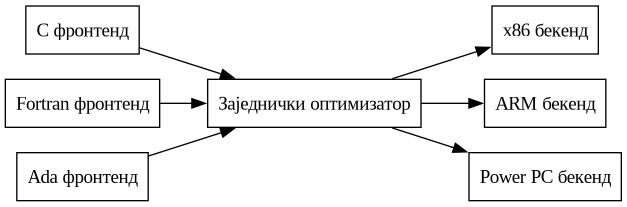
\includegraphics[width=5in, height=1.6in]{assets/images/modern_compiler_design.png}
\end{center}
\caption{Модуларност LLVM-a}
\label{lst:llvm_modular}
\end{listing}

Постоје бројне врсте оптимизације које се могу извршити над изворним кодом. Оптимизације се обично своде 
на три основна корака, проналазак шаблона који се треба трансформисати, валидирати да ли је безбедно применити 
трансформацију и извршавање трансформације \cite{oss-architecture}. Оптимизације у \verb|LLVM| оптмизатору су модуларне и извршавају 
се над \verb|LLVM| међу репрезентацијом. Свака \verb|LLVM| оптмизација је написана као \verb|C++| класа која 
наслеђује \verb|Pass| (пролазак) класу. Већина пролазака је написана у једаном \verb|.cpp| фајлу.
Стога отвара се могућност да се додају оптимизације специфичне за језик. Сваки пролазак се компајлира у један 
или више релокатабилних објеката, (\verb|.o|) фајлова који се потом групишу у архивне (\verb|.a|) фајлове. Објектни фајлови 
су машински код пре процеса линковања. Линковање је процес скупљања и комбиновања релокатабилних објектних фајлова
у један извршни објектни фајл. Приликом линковања неког \verb|.o| фајла са \verb|.a| фајлом линкер ће 
за сваки до тада неспојен симбол пробати да нађе везу у свим \verb|.o| фајловима архиве.

\verb|LLVM| генератор кода је одговаран за превођење \verb|LLVM| међу репрезентације у машински код циљане 
архитектуре. Идеално за сваку архитектуру постојао би специфичан код за превођење, али у исто време 
сви генератори раде врло сличан посао. Слично као и код оптимизације процес генерисања кода се дели у проласке,
избор сета инструкција, начин алокације регистара, планирање (\verb|scheduling|), оптимизација распореда 
кода и генерисање асемблерског кода. При креирању генератора за нову циљну архитектуру сваки од ових пролазака
може поново да се искористи, модификује или потпуно замени.

\verb|LLVM| међу репрезентација се веома ефикасно серијализује у и десериализује из \verb|LLVM| биткода. 
Ова ефикасност отвара могућност за оптимизацију у време линковања \ref{lst:link_time_opt}. То је још један сет оптимизационих пролазака 
који додатно побољшава крањи машински код. Линкер препознаје да се у \verb|.o| фајловима налази 
\verb|LLVM| биткод уместо машинског кода, учитава их у меморију, линкује их, а потом извршава \verb|LLVM|
оптимизатор над много већом целином кода, омогућавајући далеко агресивније оптимизације. 
Ова опција се укључује додавањем \verb|-O4| опције командне линије. 

\begin{listing}[H]
\begin{center}
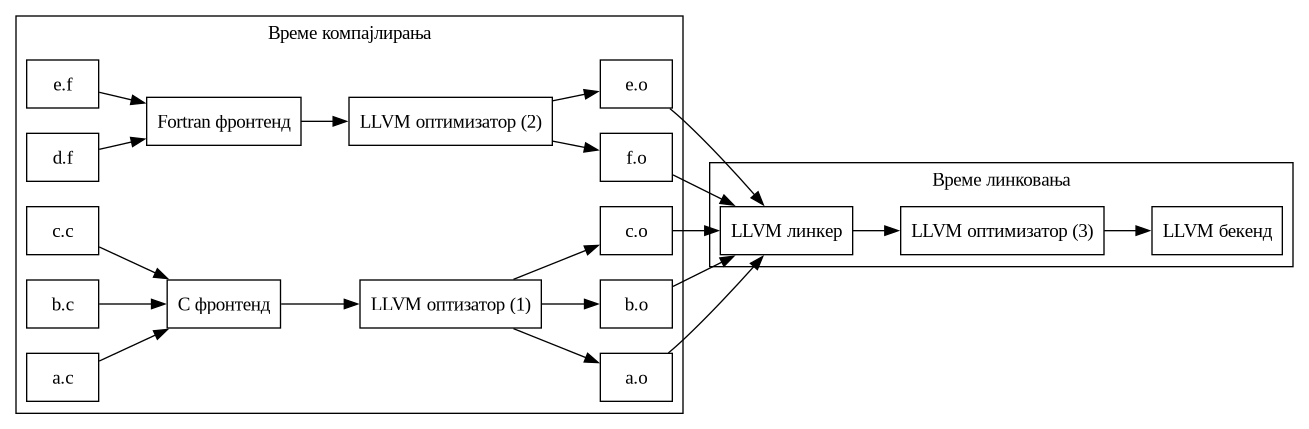
\includegraphics[width=6in, height=2.2in]{assets/images/link_time_optimization.png}
\end{center}
\caption{Оптимизација у време линковања}
\label{lst:link_time_opt}
\end{listing}

\verb|LLVM| међу репрезентација подесћа на асемблерски језик. Строго је типизиран и поседује једноставне 
типове попут целих бројева, бројева са покретним зарезом, показивача и структура. Једна од главних разлика 
у односу на асемблер јесте то што не користи ограничени број именованих регистара већ користи бесконачан 
скуп променљивих које се дефинишу са \verb|%| префиксом. Неки детаљи машине су апстраховани од корисника 
попут позива функција (\verb|call|) и враћања вредности (\verb|ret|) \ref{lst:llvm_ir}.

\begin{listing}[H]
\begin{minted}{llvm}
define i32 @add2(i32 %a, i32 %b) {
entry:
  %tmp1 = icmp eq i32 %a, 0
  br i1 %tmp1, label %done, label %recurse

recurse:
  %tmp2 = sub i32 %a, 1
  %tmp3 = add i32 %b, 1
  %tmp4 = call i32 @add2(i32 %tmp2, i32 %tmp3)
  ret i32 %tmp4

done:
  ret i32 %b
}
\end{minted}
\caption{LLVM међурепрезентација}
\label{lst:llvm_ir}
\end{listing}

\verb|Rust| језик је \verb|frontend| над \verb|LLVM|-ом. Постоји пуно олакшица у овом приступу.
\verb|Rust| тим има циљ да изгенерише правилну \verb|LLVM| међурепрезентацију, на основу које 
\verb|LLVM| извршава оптимизационе проласке и генерише код. Грешке приликом генерисања кода не мора да 
одржава \verb|Rust| тим, што значајно смањује количину људи која активно мора да буде укључена у развој. 
Свака циљна дистрибуција (архитектура) коју \verb|LLVM| подржава аутоматски подржава и \verb|Rust|. Оптимизације се не морају 
посебно писати и одржавати јер \verb|LLVM| већ поседује значајан број честих оптимизација. \verb|Rust| 
омогућава компајлирање на основу више \verb|LLVM| верзија, последња главна верзија је увек подржана,
и обично су подржане једна или две испод ње.
